% $Id: browsers.tex 8161 2009-04-06 14:07:39Z alexandra $
% Local Variables:
% ispell-check-comments: nil
% Local IspellDict: american
% End:
% --------------------------------------------------------
% User documentation
% copyright by BREDEX GmbH 2004
% --------------------------------------------------------
\index{Browser!Test Suite}
\index{Browser!Test Case}

There are three browsers in \app{}:
\begin{description}
\item[The \gdtestcasebrowser{}]{ lets you create and manage your \gdcases{}. }
\item[The \gdtestsuitebrowser{}]{ lets you create and manage your \gdsuites{}.}
\item [The \gdcompnamebrowser{}]{lets you see, merge add and delete component names.}
\end{description}

\subsection{The \gdtestsuitebrowser{}}
\gdhelpid{testExecutionViewContextId}{Test Suite Browser}
The \gdtestsuitebrowser{} is by default in the upper left-hand corner of the \specpersp{}. In this browser, you can create \gdsuites{} and \gdjobs{} for executing tests. 

More information on working with browsers is available in the Tasks chapter \bxpref{WorkingWithBrowsers}.

\bxtipp{You can filter in the \gdtestsuitebrowser{} using the field at the top. Use star \bxshell{*} as a wild card.}

\subsection{The \gdtestcasebrowser{}}
\gdhelpid{testSpecificationViewContextId}{Test Case Browser}

The \gdtestcasebrowser{} is by default in the lower left-hand corner of the \specpersp{}. In this browser, you can create \gdcases{}, which are the ''building blocks'' in \app{}. They are used to group \gdsteps{} and other \gdcases{}.  

More information on working with browsers is available in the Tasks chapter \bxpref{WorkingWithBrowsers}. To make working with larger \gdprojects{} easier, you can also have the \gdtestcasebrowser{} open more than once \bxpref{TasksMultipleTCB}.

\bxtipp{You can filter in the \gdtestcasebrowser{} using the field at the top. Use star \bxshell{*} as a wild card.}

\subsection{The \gdcompnamebrowser}
\gdhelpid{guidancerComponentNameBrowserContextId}{Component Name Browser}

The \gdcompnamebrowser{} (\bxfigref{compnamesbrowser}) is by default in the lower left-hand corner of the \specpersp{}, behind the \gdtestcasebrowser{}. In this browser, you can see component names used in this \gdproject{} and in other \gdprojects{}. You can rename, add, delete and merge component names and can also find where you have used component names in your test. 
 
\bxtipp{You can filter in the \gdcompnamebrowser{} using the field at the top. Use star \bxshell{*} as a wild card.}

\begin{figure}[h]
\begin{center}
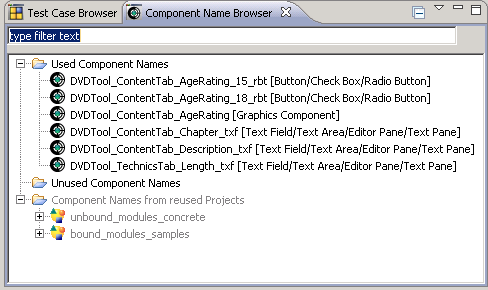
\includegraphics{Userinterface/Editors/PS/compnamesbrowser}
\caption{Component Name Browser}
\label{compnamesbrowser}
\end{center}
\end{figure}
